\PrestigeClass[\subsectionA][\subsubsection]{Athasian Dragon}
{The Dragon of Tyr is a true legend, a reptilian beast unrivaled in power and terrible evil. It claims a thousand lives every time it visits our great city. On decree of our god-king, a thousand slaves are sent to their deaths at the claws of the beast. This is not an honorable death, son, thus we despise the dragon and curse the silt it crosses to get here.}
{A Draji father to his son.}
{
Dragons are incredibly powerful individuals who have mastered both arcane magic and psionics. In their quests for power, these individuals have chosen to undergo a metamorphosis, changing them into reptilian dragons.

Dragons command terrible magic capable of draining the life-force of both man and beast, leaving only withered skulls behind. They are masters of the Way and the arcane arts, which can combine these supernatural powers into psionic enchantments, allowing them to exploit even further might.
}
{d12}
{a}
{
Only an epic spellcaster with a fairly high manifester level can qualify to become an Athasian dragon. Dragons use psionics to focus their minds in order to go through the metamorphosis, so because of the rigorous dedication in studying the processes, wilders likewise rarely become dragons. Some dragons take levels of cerebremancer to boost both their arcane and psionic skills.
}
{
\textbf{Skills:} \skill{Knowledge} (arcana) 23 ranks, \skill{Knowledge} (ancient history) 23 ranks, \skill{Knowledge} (psionics) 23 ranks, \skill{Psicraft} 23 ranks, \skill{Spellcraft} 23 ranks.

\textbf{Feats:} \feat{Mind Over Body}, any one raze feat, any two metamagic feats, and any two psionic feats.

\textbf{Spells:} Able to cast 9th-level arcane spells.

\textbf{Psionics:} Able to manifest 7th-level powers.

\textbf{Special:} Must be a defiler.

\textbf{Special:} Must perform a special ritual (see \hyperref[Defiler Metamorphosis]{Defiler Metamorphosis}).
}
{
\skill{Concentration} (Con), \skill{Craft} (Int), \skill{Decipher Script} (Int), \skill{Diplomacy} (Cha), \skill{Knowledge} (all skills, taken separately) (Int), \skill{Psicraft} (Int), \skill{Sense Motive} (Wis), and \skill{Spellcraft} (Int).
}
{2}
{\WarriorTable[ll *{3}{Z{12mm}} L]}
{
 1 & +1  & +2 & +2 & +2 & Continued advancement, divine rank, \spell{tongues}          \\
 2 & +2  & +3 & +3 & +3 & Increased size                                               \\
 3 & +3  & +3 & +3 & +3 & Frightful presence, natural attack (claws)                   \\
 4 & +4  & +4 & +4 & +4 & Improved speed, natural armor                                \\
 5 & +5  & +4 & +4 & +4 & DR 10/metal and magic, increased size, natural attack (bite) \\
 6 & +6  & +5 & +5 & +5 & Resistance                                                   \\
 7 & +7  & +5 & +5 & +5 & Breath (10d12)                                               \\
 8 & +8  & +6 & +6 & +6 & DR 20/metal and epic, increased size, natural attack (tail)  \\
 9 & +9  & +6 & +6 & +6 & Breath (20d12), natural attack (wings)                       \\
10 & +10 & +7 & +7 & +7 & Draconic perfection                                          \\
}
{
\textbf{Continued Advancement:} When a new dragon level is attained, the character gains new spells per day as if he had also attained a level in any one arcane spellcasting class he belonged to before he added the prestige class. He gains additional power points per day and access to new powers as if he had also gained a level in any one manifesting class he belonged to previously. He does not, however, gain any other benefit a character of either class would have gained (bonus metamagic, metapsionic, or item creation feats, psicrystal special abilities, and so on). This essentially means that he adds the level of dragon to the level of whatever other arcane spellcasting class and manifesting class the character has, then determines spells per day, caster level, power points per day, powers known, and manifester level accordingly.

If a character had more than one arcane spellcasting class or more than one manifesting class before he became a dragon, he must decide to which class he adds each level of dragon for purpose of determining spells per day, caster level, power points per day, powers known, and manifester level.

\textbf{Divine Rank:} A dragon is considered a demigod. He can grant spells and perform a few deeds that are beyond mortal limits. He is immune to the effects of aging and never dies of ``natural causes.'' For more information, see \hyperref[Divine Rank]{Divine Rank}.

\textit{Tongues (Sp):} A dragon gains the ability to understand and speak any language, as per the \spell{tongues} spell. This spell-like ability is always considered active.

\begin{figure*}[b!]
\centering
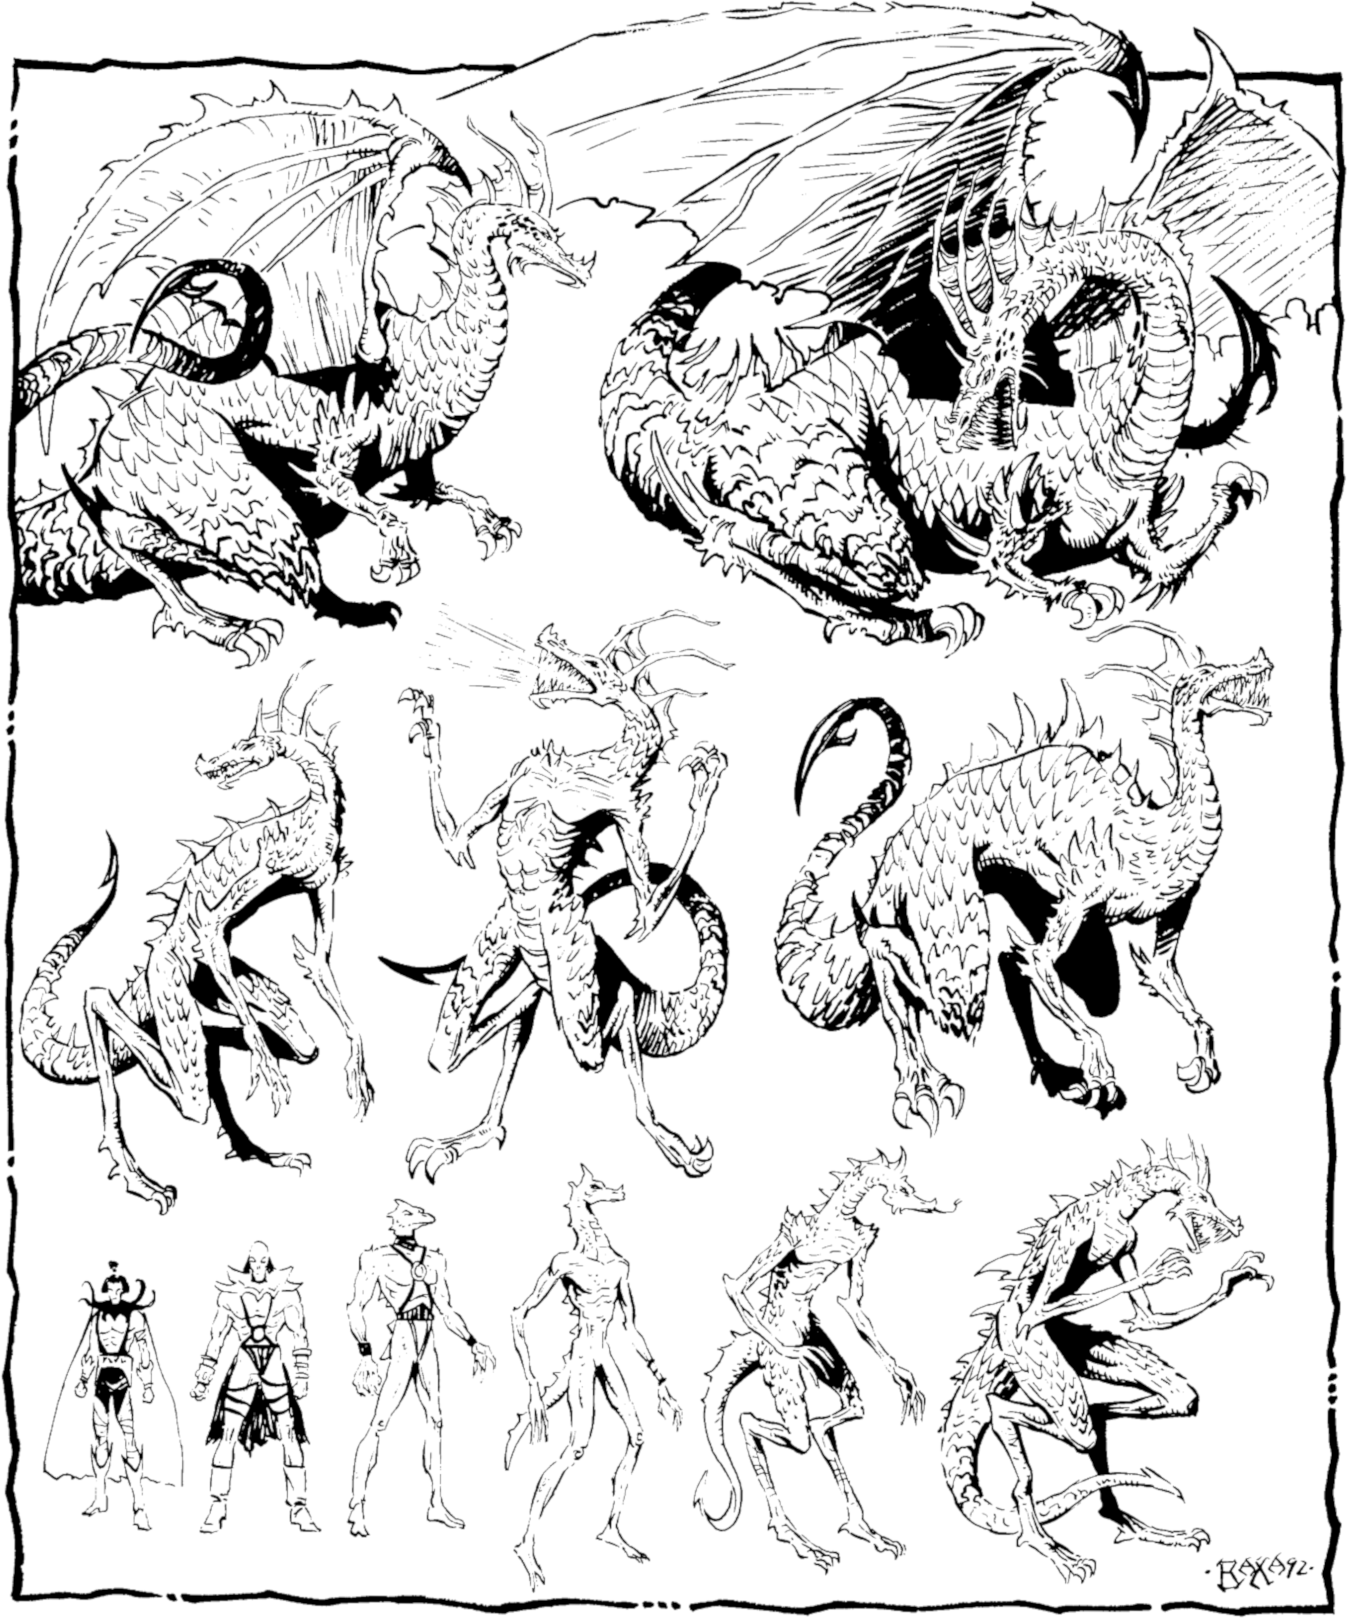
\includegraphics[width=\textwidth]{images/dragon-3.png}
\WOTC
\end{figure*}

\textbf{Increased Size:} At 2nd level and every three levels thereafter (5th and 8th level), a dragon increases in size by one category. At each size increase, the dragon improves his Strength score by 8, and his Constitution score by 4. The size indicated at the table is for Medium dragons. Small and Large dragons increase the size by one category normally. Small Dragons that become Medium improve Strength as indicated, as this is not a normal monster progression. Colossal dragons cannot increase further in size.

\textbf{Natural Attacks:} At 3rd level, a dragon begins to gain natural weapons. These natural attacks change damage with each increase in size (see \tabref{Dragon's Natural Attack Damage}). A dragon is considered proficient with these attacks.

\Table{Dragon's Natural Attack Damage}{lCCCC}{
\tableheader Level & \tableheader Claw & \tableheader Bite & \tableheader Tail & \tableheader Wings\\
 1 &     &      &     &     \\
 2 &     &      &     &     \\
 3 & 3d6 &      &     &     \\
 4 & 3d6 &      &     &     \\
 5 & 4d6 &  6d8 &     &     \\
 6 & 4d6 &  6d8 &     &     \\
 7 & 4d6 &  6d8 &     &     \\
 8 & 6d6 &  8d8 & 6d6 &     \\
 9 & 6d6 &  8d8 & 6d6 & 4d6 \\
10 & 8d6 & 10d8 & 8d6 & 6d6 \\
}

\textit{Claws:} At 3rd level, a dragon's hands become natural weapons. He gains two claw attacks that deal the indicated damage plus \onehalf the dragon's Strength bonus (round down). The dragon also can use its claws to snatch opponents if it has the \feat{Snatch} feat. Claw attacks are secondary attacks, requiring a $-5$ penalty on the attack roll. (Many dragons choose the \feat{Multiattack} feat to lessen this penalty to $-2$).

\textit{Bite:} At 5th level, a dragon's jaws protrude remarkably, allowing for a bite attack. Bite attacks deal the indicated damage plus the dragon's Strength bonus. A dragon also can use its bite to snatch opponents if it has the \feat{Snatch} feat.

\textit{Tail Slap:} At 8th level, a dragon's tail can be weaponized, as he gains a tail slap attack. The dragon can slap one opponent each round with its tail. A tail slap deals the indicated damage plus 1\onehalf times the dragon's Strength bonus (round down) and is treated as a secondary attack.

\textit{Wings:} At 9th level, a dragon grows bat-like wings. These wings grant him a flight speed of 18 meters with poor maneuverability. These wings can also be weaponized, as he gains two wing attacks. The dragon can slam opponents with its wings, even when flying. Wing attacks deal the indicated damage plus \onehalf the dragon's Strength bonus (round down) and are treated as secondary attacks.

\textbf{Frightful Presence (Ex):} At 3rd level, a dragon can unsettle foes with its mere presence. The ability takes effect automatically whenever the dragon attacks, charges, or flies overhead. Creatures within a radius of 9 meters $\times$ the dragon's level are subject to the effect if they have fewer HD than the dragon. A potentially affected creature that succeeds on a Will save (DC 10 + dragon's HD + dragon's Cha modifier) remains immune to that dragon's frightful presence for 24 hours. On a failure, creatures with 4 or less HD become panicked for 4d6 rounds and those with 5 or more HD become shaken for 4d6 rounds. Dragons ignore the frightful presence of other dragons.

\textbf{Improved Speed (Ex):} At 4th level, a dragon increases his land speed by 6 meters.

\textbf{Natural Armor:} At 4th level, tough scales, now everywhere but the underbelly and the underside of its limbs, grant a dragon natural armor equal to its level + his Intelligence modifier.

\textbf{Damage Reduction:} At 5th level, a dragon's gains damage reduction 10/metal and magic. So attacks from weapons that are not made of metal have their damage reduced, even if the weapon has an enhancement bonus. Only metal weapons with an enhancement bonus can ignore this damage reduction. Damage reduction can reduce damage to 0 but not below 0.

At 8th level, this damage reduction improves to 20/metal and epic. Only attacks with metal weapons with an enhancement bonus of +6 or better can ignore this damage reduction.

\textbf{Resistance (Su):} At 6th level, a dragon gains spell resistance and power resistance equal to 12 + dragon's HD.

\textbf{Breath Attack (Su):} At 7th level, a dragon can use its breath weapon, a cone of superheated sand 15 meters long. The cone deals 10d12 points of damage. A blast from a breath weapon always starts at any intersection adjacent to the dragon and extends in a direction of the dragon's choice. The creatures caught in the area can attempt Reflex saves to take half damage. The save DC against a breath weapon is 10 + dragon's HD + dragon's Con modifier.

At 9th level, the dragon's breath attack increases its damage to 20d12.

\textbf{Draconic Perfection:} By obtaining the 10th level, the dragon's type changes to Dragon. All of his hit dice become d12. He increases in size by one last time, and his natural attacks increase their damage because of it. His flight speed improves to 45 meters with average maneuverability. His breath attack damage increases to 25d12.

\subsubsection{The Animalistic Stages}
From 5th through 9th levels, the ascending dragon goes through a terrible rampaging period. Reason is often superseded by a lust for destruction. Vegetation and animals that do not directly serve the dragon's purpose are targets for its unending wrath, laid waste in its quest for power and advancement. The savage destruction comes of the incredible pain that wracks its body during these final stages of metamorphosis. No longer human but not yet dragon, its need to end the process nearly drives it mad.

For role-playing purposes, advancing dragons should take an illogical bent toward destruction. DMs should guide the player characters in this stage, so that the true maddening destruction can be accomplished.

\subsubsection{Defiler Metamorphosis}
\label{Defiler Metamorphosis}

In order to receive the benefits of the prestige class, a character must perform a defiling ritual to change their body. This ritual depends on the level in which the character wants to obtain. Although the experience points have been earned (or the number of sessions have been passed), the defiler gains no benefits of his new level until after the ritual is complete.

The ritual functions as a special spell of at least 9th-level that consumes all power points from the caster. It has the verbal, somatic, and material components of a normal spell, but it also requires a special component: the life of a number of living creatures. Besides, some transformations require a special structure as a arcane focus.

\textbf{Low Level (1st, 2nd, and 3rd levels):} The defiler is merely beginning his metamorphosis toward dragon form. During the preparation time of this ritual the caster must have access to ancient documents, tablets, and scrolls. Such materials must be studied for at least eight hours every day for the entire year. The ritual consumes all materials and documents, the creatures serving as living components turn to defiler ash and die and cannot be ressurrected by normal means.

\textit{Spell Level:} 9th-level.

\textit{Preparation Time:} 1 year.

\textit{Casting Time:} 24 hours.

\textit{Material Component:} Jewels, gems, coins, or artistic treasures worth at least 30,000 cp per level.

\textit{Living Component:} 1,000 Hit Dice of living creatures per level.

\textit{Arcane Focus:} A huge structure capable of holding the living components for the ritual costing at least 150,000 cp.

\textbf{Middle Level (4th, 5th, and 6th levels):} During the preparation time, the caster visits a powerful creature on an elemental plane for one day of every five.

\textit{Spell Level:} 10th-level.

\textit{Preparation Time:} 2 years.

\textit{Casting Time:} 3 days.

\textit{Material Component:} Jewels, gems, coins, or artistic treasures worth at least 15,000 cp per level.

\textit{Living Component:} 2,000 Hit Dice of living creatures per level.

\textit{Arcane Focus:} A huge structure capable of holding the living components for the ritual, different from the structure used by the low level transformations, costing at least 375,000 cp.

\textbf{High Level (7th, 8th, and 9th levels):} The high levels of dragon metamorphosis must take place on either an Elemental or the Astral Plane. No structure or riches are requires, but the caster must travel to the plane of choice with the living components from the Material Plane. At least three powerful beings from that plane must cooperate with the casting of the spell, so the preparation time is equal to the time it takes to convince the planar beings to cooperate.

\textit{Spell Level:} 10th-level.

\textit{Preparation Time:} Special (see above).

\textit{Casting Time:} 24 hours.

\textit{Living Component:} 200 Hit Dice of living creatures per level, with at least 10 HD each.

\textbf{Final Level (10th level):} The final stage of dragon metamorphosis requires no preparation time and a single material component: the slain body of a good spellcaster. The spell must be cast over the fallen victim within one hour of his defeat.

\textit{Spell Level:} 10th-level.

\textit{Casting Time:} 1 full round.

\textit{Material Component:} The slain body of a good spellcaster with at least 20 Hit Dice, capable of casting 9th-level spells, slain in single combat.

}